\documentclass{article}\usepackage[]{graphicx}\usepackage[]{xcolor}
% maxwidth is the original width if it is less than linewidth
% otherwise use linewidth (to make sure the graphics do not exceed the margin)
\makeatletter
\def\maxwidth{ %
  \ifdim\Gin@nat@width>\linewidth
    \linewidth
  \else
    \Gin@nat@width
  \fi
}
\makeatother

\definecolor{fgcolor}{rgb}{0.345, 0.345, 0.345}
\newcommand{\hlnum}[1]{\textcolor[rgb]{0.686,0.059,0.569}{#1}}%
\newcommand{\hlsng}[1]{\textcolor[rgb]{0.192,0.494,0.8}{#1}}%
\newcommand{\hlcom}[1]{\textcolor[rgb]{0.678,0.584,0.686}{\textit{#1}}}%
\newcommand{\hlopt}[1]{\textcolor[rgb]{0,0,0}{#1}}%
\newcommand{\hldef}[1]{\textcolor[rgb]{0.345,0.345,0.345}{#1}}%
\newcommand{\hlkwa}[1]{\textcolor[rgb]{0.161,0.373,0.58}{\textbf{#1}}}%
\newcommand{\hlkwb}[1]{\textcolor[rgb]{0.69,0.353,0.396}{#1}}%
\newcommand{\hlkwc}[1]{\textcolor[rgb]{0.333,0.667,0.333}{#1}}%
\newcommand{\hlkwd}[1]{\textcolor[rgb]{0.737,0.353,0.396}{\textbf{#1}}}%
\let\hlipl\hlkwb

\usepackage{framed}
\makeatletter
\newenvironment{kframe}{%
 \def\at@end@of@kframe{}%
 \ifinner\ifhmode%
  \def\at@end@of@kframe{\end{minipage}}%
  \begin{minipage}{\columnwidth}%
 \fi\fi%
 \def\FrameCommand##1{\hskip\@totalleftmargin \hskip-\fboxsep
 \colorbox{shadecolor}{##1}\hskip-\fboxsep
     % There is no \\@totalrightmargin, so:
     \hskip-\linewidth \hskip-\@totalleftmargin \hskip\columnwidth}%
 \MakeFramed {\advance\hsize-\width
   \@totalleftmargin\z@ \linewidth\hsize
   \@setminipage}}%
 {\par\unskip\endMakeFramed%
 \at@end@of@kframe}
\makeatother

\definecolor{shadecolor}{rgb}{.97, .97, .97}
\definecolor{messagecolor}{rgb}{0, 0, 0}
\definecolor{warningcolor}{rgb}{1, 0, 1}
\definecolor{errorcolor}{rgb}{1, 0, 0}
\newenvironment{knitrout}{}{} % an empty environment to be redefined in TeX

\usepackage{alltt}
\usepackage[margin=1.0in]{geometry} % To set margins
\usepackage{amsmath}  % This allows me to use the align functionality.
        % If you find yourself trying to replicate
        % something you found online, ensure you're
        % loading the necessary packages!
\usepackage{amsfonts} % Math font
\usepackage{fancyvrb}
\usepackage{xcolor}
\usepackage{hyperref} % For including hyperlinks
\usepackage[shortlabels]{enumitem}% For enumerated lists with labels specified
                    % We had to run tlmgr_install("enumitem") in R
\usepackage{float}    % For telling R where to put a table/figure
\usepackage{natbib}        %For the bibliography
\bibliographystyle{apalike}%For the bibliography
\IfFileExists{upquote.sty}{\usepackage{upquote}}{}
\begin{document}
\noindent\textbf{Homework 2: Exploring One Sample Inference}\\
\noindent\makebox[\linewidth]{\rule{\textwidth}{0.4pt}}
\noindent\underline{Submission Notes:} Please write your answers to each 
question under that question (not altogether at the end). It will be easier for 
me to give full credit if your answer is commented well, including comments 
about where you are completing each sub-part of the question. For an example,
see Homework 1.\\
\noindent\makebox[\linewidth]{\rule{\textwidth}{0.4pt}}

\begin{enumerate}
  %%%%%%%%%%%%%%%%%%%%%%%%%%%%%%%%%%%%%%%%%%%%%%%%%%%%%%%%%%%%%%%%%%%%%%%%%%%%%%%%
  %%%%%%%%%%%%%%%%%%%%%%%%%%%%%%%%%%%%%%%%%%%%%%%%%%%%%%%%%%%%%%%%%%%%%%%%%%%%%%%%
  % Question 1
  %%%%%%%%%%%%%%%%%%%%%%%%%%%%%%%%%%%%%%%%%%%%%%%%%%%%%%%%%%%%%%%%%%%%%%%%%%%%%%%%
  %%%%%%%%%%%%%%%%%%%%%%%%%%%%%%%%%%%%%%%%%%%%%%%%%%%%%%%%%%%%%%%%%%%%%%%%%%%%%%%%
  \item Complete the following to explore differences in tests that use discrete 
  (versus continuous) sampling distributions. In both parts (a) and (b), assume
  we aim to conduct the following test:
  \begin{align*}
    H_0&: p = 0.50\\
    H_a&: p < 0.50
  \end{align*}
  \begin{enumerate}
    \item A Binomial Test under the condition that we plan to obtain $n=15$ 
    observations.
    \begin{enumerate}
      \item Plot a Binomial($n=15$, $p=0.50$) distribution.
      
      \begin{figure}[H]
\begin{knitrout}\scriptsize
\definecolor{shadecolor}{rgb}{0.969, 0.969, 0.969}\color{fgcolor}\begin{kframe}
\begin{alltt}
\hlkwd{library}\hldef{(ggplot2)}
\hlkwd{library}\hldef{(tidyverse)}

\hldef{n} \hlkwb{=} \hlnum{15} \hlcom{#our sample size}

\hldef{p} \hlkwb{=} \hlnum{0.5} \hlcom{#our hypothesis probability}

\hlcom{#Create tibble of associated probabilities of each observation under the binomial distribution}
\hldef{ggdat} \hlkwb{<-} \hlkwd{tibble}\hldef{(}\hlkwc{x} \hldef{=} \hlnum{1}\hlopt{:}\hldef{n,}
                \hlkwc{p} \hldef{=} \hlkwd{dbinom}\hldef{(}\hlnum{1}\hlopt{:}\hldef{n,}\hlkwc{size} \hldef{= n,} \hlkwc{p} \hldef{= p))}

\hlkwd{ggplot}\hldef{(}\hlkwc{data} \hldef{= ggdat,} \hlkwd{aes}\hldef{(}\hlkwc{x} \hldef{= x,} \hlkwc{y} \hldef{= p))} \hlopt{+}
  \hlkwd{geom_linerange}\hldef{(}\hlkwd{aes}\hldef{(}\hlkwc{ymin} \hldef{=} \hlnum{0}\hldef{,} \hlkwc{ymax} \hldef{= p),} \hlkwc{linewidth} \hldef{=} \hlnum{3}\hldef{)} \hlopt{+}
  \hlkwd{theme_bw}\hldef{()} \hlopt{+}
  \hlkwd{geom_hline}\hldef{(}\hlkwc{yintercept} \hldef{=} \hlnum{0}\hldef{)} \hlopt{+}
  \hlkwd{ylab}\hldef{(}\hlsng{'density'}\hldef{)} \hlopt{+}
  \hlkwd{labs}\hldef{(}\hlkwc{subtitle} \hldef{=} \hlsng{'n = 15, p = 0.50'}\hldef{)} \hlopt{+}
  \hlkwd{xlim}\hldef{(}\hlnum{0}\hldef{,}\hlnum{15}\hldef{)}
\end{alltt}
\end{kframe}
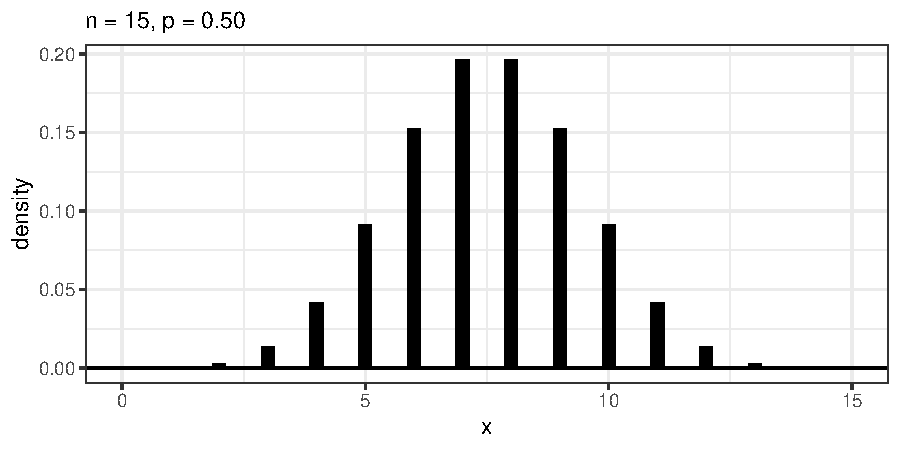
\includegraphics[width=\maxwidth]{figure/unnamed-chunk-1-1} 
\end{knitrout}
      
      \label{binom_dist}
      \caption{Binomial Distribution Plot}
      
      \end{figure}
      
      \item What is the $\alpha=0.05$ percentile from this distribution?
      
\begin{knitrout}\scriptsize
\definecolor{shadecolor}{rgb}{0.969, 0.969, 0.969}\color{fgcolor}\begin{kframe}
\begin{alltt}
\hldef{alpha} \hlkwb{=} \hlnum{0.05} \hlcom{#intended alpha}
\hlkwd{qbinom}\hldef{(}\hlkwc{p} \hldef{= alpha,} \hlkwc{size} \hldef{= n,} \hlkwc{prob} \hldef{= p)} \hlcom{#inverse cdf to find 5th percentile observation}
\end{alltt}
\begin{verbatim}
## [1] 4
\end{verbatim}
\end{kframe}
\end{knitrout}
      
      \textcolor{red}{The $\alpha = 0.05$ percentile from this distribution is 4 according to $qbinom$.}
      
      \[b_\alpha = F_B^{-1}(\alpha)\]
      \item Compute $P(B \leq b_\alpha)$. Is it in the rejection region?
      
\begin{knitrout}\scriptsize
\definecolor{shadecolor}{rgb}{0.969, 0.969, 0.969}\color{fgcolor}\begin{kframe}
\begin{alltt}
      \hlkwd{pbinom}\hldef{(}\hlkwc{q} \hldef{=} \hlnum{4}\hldef{,} \hlkwc{size} \hldef{= n,} \hlkwc{prob} \hldef{= p)}
\end{alltt}
\begin{verbatim}
## [1] 0.05923462
\end{verbatim}
\begin{alltt}
      \hlcom{# find the associated probability of observing 4 or fewer from our null distribution}
\end{alltt}
\end{kframe}
\end{knitrout}
      
      \textcolor{red}{It is not in the rejection region because it is not less than 0.05.}
      
      \item What is the largest observation in the rejection region?
      
\begin{knitrout}\scriptsize
\definecolor{shadecolor}{rgb}{0.969, 0.969, 0.969}\color{fgcolor}\begin{kframe}
\begin{alltt}
      \hlkwd{pbinom}\hldef{(}\hlkwc{q} \hldef{=} \hlnum{3}\hldef{,} \hlkwc{size} \hldef{= n,} \hlkwc{prob} \hldef{= p)} \hlcom{# Test out 3}
\end{alltt}
\begin{verbatim}
## [1] 0.01757813
\end{verbatim}
\end{kframe}
\end{knitrout}
      
      \textcolor{red}{3 is the largest observation in the rejection region.}
      
      \item What is the achieved $\alpha$ for this test? That is, what 
      is the probability of a Type I error for this specification?
      
        \textcolor{red}{The achieved $\alpha$ is 0.018, because that is essentially our threshold for significance when the largest rejectable value has that probability associated.}
      
    \end{enumerate}
    \item A $z$-test.
    \begin{enumerate}
      \item Plot the standard Gaussian distribution.
      
            \begin{figure}[H]
\begin{knitrout}\scriptsize
\definecolor{shadecolor}{rgb}{0.969, 0.969, 0.969}\color{fgcolor}\begin{kframe}
\begin{alltt}
\hlcom{# create tibble of gaussian densities}
\hldef{gaussian_dat} \hlkwb{<-} \hlkwd{tibble}\hldef{(}\hlkwc{x} \hldef{=} \hlkwd{seq}\hldef{(}\hlkwc{from} \hldef{=} \hlopt{-}\hlnum{5}\hldef{,}
                               \hlkwc{to} \hldef{=} \hlnum{5}\hldef{,}
                               \hlkwc{length.out} \hldef{=} \hlnum{10000}\hldef{),}
                       \hlkwc{d} \hldef{=} \hlkwd{dnorm}\hldef{(}\hlkwd{seq}\hldef{(}\hlkwc{from} \hldef{=} \hlopt{-}\hlnum{5}\hldef{,}
                                     \hlkwc{to} \hldef{=} \hlnum{5}\hldef{,}
                                     \hlkwc{length.out} \hldef{=} \hlnum{10000}\hldef{)))}

\hlkwd{ggplot}\hldef{(}\hlkwc{data} \hldef{= gaussian_dat,} \hlkwd{aes}\hldef{(}\hlkwc{x} \hldef{= x,} \hlkwc{y} \hldef{= d))} \hlopt{+} \hlkwd{geom_line}\hldef{()} \hlopt{+}
  \hlkwd{theme_bw}\hldef{()} \hlopt{+}
  \hlkwd{xlab}\hldef{(}\hlsng{'Z'}\hldef{)} \hlopt{+}
  \hlkwd{ylab}\hldef{(}\hlsng{'density'}\hldef{)} \hlopt{+}
  \hlkwd{geom_hline}\hldef{(}\hlkwc{yintercept} \hldef{=} \hlnum{0}\hldef{)}
\end{alltt}
\end{kframe}
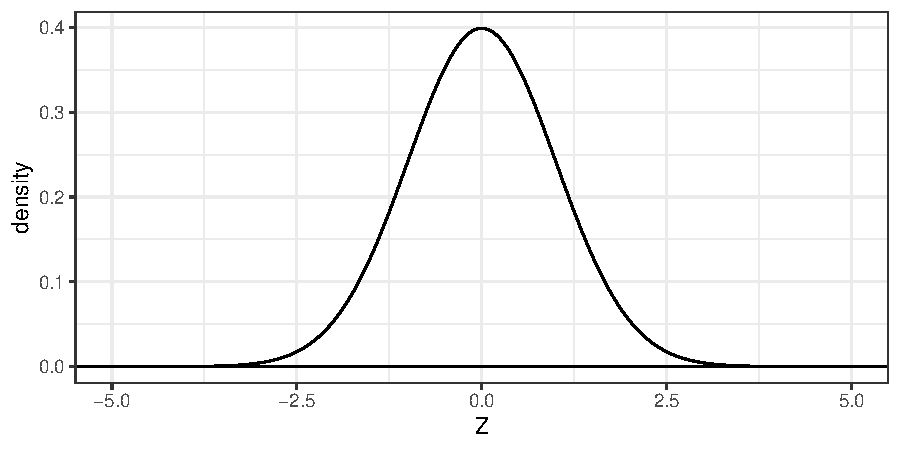
\includegraphics[width=\maxwidth]{figure/unnamed-chunk-5-1} 
\end{knitrout}
      
      \label{gaussian_dist}
      \caption{Gaussian Distribution Plot}
      
      \end{figure}
      
      \item What is the $\alpha=0.05$ percentile from this distribution?
      \[z_\alpha = F_Z^{-1}(\alpha)\]
      
\begin{knitrout}\scriptsize
\definecolor{shadecolor}{rgb}{0.969, 0.969, 0.969}\color{fgcolor}\begin{kframe}
\begin{alltt}
      \hldef{fifth_percentile} \hlkwb{<-} \hlkwd{qnorm}\hldef{(}\hlkwc{p} \hldef{= alpha)}

      \hldef{fifth_percentile}
\end{alltt}
\begin{verbatim}
## [1] -1.644854
\end{verbatim}
\end{kframe}
\end{knitrout}
      
      \textcolor{red}{The 5th percentile observation is -1.645 standard deviations from the mean.}
      
      \item Compute $P(Z \leq z_\alpha)$. Is it in the rejection region?
      
\begin{knitrout}\scriptsize
\definecolor{shadecolor}{rgb}{0.969, 0.969, 0.969}\color{fgcolor}\begin{kframe}
\begin{alltt}
      \hlkwd{pnorm}\hldef{(}\hlkwc{q} \hldef{= fifth_percentile)}
\end{alltt}
\begin{verbatim}
## [1] 0.05
\end{verbatim}
\end{kframe}
\end{knitrout}
      
      \textcolor{red}{Technically this observation is not in the rejection region, as we would consider anything with a probability of \textless 0.05.}
      
      \item What is the largest observation in the rejection region?\\
      
      \textbf{Hint:} We know $z$, $n$ and $p_0$, solve for $\hat{p}$.
      
      \[Z = \frac{\hat{p} - p_{0}}{\sqrt{p_{0}(1-p_{0})/n}} \]
      
      \[-1.644854 \textgreater \frac{\hat{p} - 0.5}{\sqrt{0.5(1-0.5)/15}} \]
      
      \[-1.644854 \textgreater \frac{\hat{p} - 0.5}{0.129099} \]
      
      \[-0.212350 \textgreater \hat{p} - 0.5 \]
            
      \[0.287650 \textgreater \hat{p} \]
      
      \[\frac{4}{15} = 0.2\bar{6} \]
      
      \textcolor{red}{A proportion \textless 0.287650 would be in the rejection region. The largest observation given $n = 15$ would be 4.}
      
      \item What is the achieved $\alpha$ for this test? That is, what 
      is the probability of a Type I error for this specification?
      
\begin{knitrout}\scriptsize
\definecolor{shadecolor}{rgb}{0.969, 0.969, 0.969}\color{fgcolor}\begin{kframe}
\begin{alltt}
      \hldef{p.hat} \hlkwb{=} \hlnum{4}\hlopt{/}\hlnum{15}
      \hldef{p0} \hlkwb{=} \hlnum{0.5}
      \hldef{n} \hlkwb{=} \hlnum{15}

      \hldef{(z.stat} \hlkwb{<-} \hldef{(p.hat} \hlopt{-} \hldef{p0)}\hlopt{/}\hlkwd{sqrt}\hldef{(p0}\hlopt{*}\hldef{(}\hlnum{1}\hlopt{-}\hldef{p0)}\hlopt{/}\hldef{n))}
\end{alltt}
\begin{verbatim}
## [1] -1.807392
\end{verbatim}
\begin{alltt}
      \hlkwd{pnorm}\hldef{(}\hlkwc{q} \hldef{= z.stat)}
\end{alltt}
\begin{verbatim}
## [1] 0.03535057
\end{verbatim}
\end{kframe}
\end{knitrout}
      
      \textcolor{red}{The achieved $\alpha$ for this test is approximately 0.035.}
      
      
    \end{enumerate}
  \end{enumerate}
  %%%%%%%%%%%%%%%%%%%%%%%%%%%%%%%%%%%%%%%%%%%%%%%%%%%%%%%%%%%%%%%%%%%%%%%%%%%%%%%%
  %%%%%%%%%%%%%%%%%%%%%%%%%%%%%%%%%%%%%%%%%%%%%%%%%%%%%%%%%%%%%%%%%%%%%%%%%%%%%%%%
  % Question 2
  %%%%%%%%%%%%%%%%%%%%%%%%%%%%%%%%%%%%%%%%%%%%%%%%%%%%%%%%%%%%%%%%%%%%%%%%%%%%%%%%
  %%%%%%%%%%%%%%%%%%%%%%%%%%%%%%%%%%%%%%%%%%%%%%%%%%%%%%%%%%%%%%%%%%%%%%%%%%%%%%%%
  \item Suppose we have data that follow an exponential distribution, i.e.,
  \[X_1, X_2, ..., X_n \sim \text{Exponential}(\lambda).\]
  When $n$ is large, we can employ the Central Limit Theorem to assert
  the following approximation
  \[T = \frac{\bar{X}-\lambda}{s/\sqrt{n}} \sim \mathcal{AT}(v=n-1).\]
  Recall that this approximation is ``good" when $n$ is large and the underlying 
  population distribution is more symmetric. The skewness of the Exponential 
  distribution is 2, regardless of $\lambda$, so the approximation really leans
  on the sample size in this case.
  
  Conveniently, when the population distribution is Exponential, mathematical 
  statisticians can derive the \emph{exact} sampling distribution of $\bar{X}$,
  \[\bar{X} \sim \textrm{Gamma}\left(\alpha=n, \beta=\frac{n}{\lambda}\right).\]
  If you don't want to take my word for it, see the small simulation below where 
  $n=10$ and $\lambda=2$.


  \begin{figure}[H]
    \centering
\begin{knitrout}
\definecolor{shadecolor}{rgb}{0.969, 0.969, 0.969}\color{fgcolor}

\includegraphics[width=\maxwidth]{figure/unnamed-chunk-10-1} 
\end{knitrout}
    \caption{A simulation showing that even for small $n$ the exact Gamma sampling
    distribution fits well.}
  \end{figure}
  How can I use the Gamma sampling distribution to derive an exact test 
  for $\mu_X=E(X)=\lambda$ when we assume the population distribution is 
  Exponential?
  \begin{enumerate}
    \item What should the hypotheses be? Assume a two-sided test.
    \textcolor{red}{
    \[H_{0}: \bar{X} = \lambda = \lambda_{0} \]
    \[H_{a}: \bar{X} = \lambda \neq \lambda_{0} \]
    }
    \item What should the test statistic be?
    
    \textcolor{red}{The test statistic would be $\bar{X}$.}
    
    \item What is the sampling distribution of the statistic under the null hypothesis?
    
    \textcolor{red}{The sampling distribution of $\bar{X}$ under $H_{0}$ is a Gamma distribution with $\alpha = n$ and $\beta = \frac{n}{\lambda_{0}}$.}
    
    \item What values of $\bar{X}$ provide statistically discernible support 
    for the alternative hypothesis?
    
    \textcolor{red}{Values of $\bar{X}$ that provide statistically discernible support for $H_{a}$ would be those with which the cumulative probability under the null distribution of observing such an $\bar{X}$ or more extreme is $< \frac{\alpha}{2}$ (for a two sided test).}
    
    \item How would you compute the $p$-value?
    
    \textcolor{red}{For a two sided test, an approximate method would be to double the p-value you got from a function like $pgamma()$. There's no way to exactly count it because the Gamma distribution is non-symmetric, so for a more applicable method I'd use randomization testing or bootstrapping.}
    
  \end{enumerate}
  %%%%%%%%%%%%%%%%%%%%%%%%%%%%%%%%%%%%%%%%%%%%%%%%%%%%%%%%%%%%%%%%%%%%%%%%%%%%%%%%
  %%%%%%%%%%%%%%%%%%%%%%%%%%%%%%%%%%%%%%%%%%%%%%%%%%%%%%%%%%%%%%%%%%%%%%%%%%%%%%%%
  % Question 3
  %%%%%%%%%%%%%%%%%%%%%%%%%%%%%%%%%%%%%%%%%%%%%%%%%%%%%%%%%%%%%%%%%%%%%%%%%%%%%%%%
  %%%%%%%%%%%%%%%%%%%%%%%%%%%%%%%%%%%%%%%%%%%%%%%%%%%%%%%%%%%%%%%%%%%%%%%%%%%%%%%%
  \item Compute the probability we make an observation in the rejection region
  when $\lambda=2$ and $n=10$ under the following conditions.
  \begin{enumerate}
    \item When $\lambda=2$, what is the probability we make an observation below the 2.5th percentile or above the 97.5th percentile (as computed 
    in Question 2)? 
    
\begin{knitrout}\scriptsize
\definecolor{shadecolor}{rgb}{0.969, 0.969, 0.969}\color{fgcolor}\begin{kframe}
\begin{alltt}
\hldef{n} \hlkwb{=} \hlnum{10}
\hldef{lambda} \hlkwb{=} \hlnum{2}

\hldef{low_percentile} \hlkwb{=} \hlnum{0.025}
\hldef{high_percentile} \hlkwb{=} \hlnum{0.975}

\hldef{(low_percentile_value} \hlkwb{<-} \hlkwd{qgamma}\hldef{(}\hlkwc{p} \hldef{= low_percentile,} \hlkwc{shape} \hldef{= n,} \hlkwc{rate} \hldef{= n}\hlopt{/}\hldef{lambda))}
\end{alltt}
\begin{verbatim}
## [1] 0.9590777
\end{verbatim}
\begin{alltt}
\hldef{(p_low_percentile} \hlkwb{<-} \hlkwd{mean}\hldef{(xbar}\hlopt{<}\hldef{low_percentile_value))}
\end{alltt}
\begin{verbatim}
## [1] 0.0253
\end{verbatim}
\begin{alltt}
\hldef{(high_percentile_value} \hlkwb{<-} \hlkwd{qgamma}\hldef{(}\hlkwc{p} \hldef{= high_percentile,} \hlkwc{shape} \hldef{= n,} \hlkwc{rate} \hldef{= n}\hlopt{/}\hldef{lambda))}
\end{alltt}
\begin{verbatim}
## [1] 3.416961
\end{verbatim}
\begin{alltt}
\hldef{(p_high_percentile} \hlkwb{<-} \hlkwd{mean}\hldef{(xbar}\hlopt{>}\hldef{high_percentile_value))}
\end{alltt}
\begin{verbatim}
## [1] 0.0239
\end{verbatim}
\begin{alltt}
\hldef{(p_low_percentile} \hlopt{+} \hldef{p_high_percentile)}
\end{alltt}
\begin{verbatim}
## [1] 0.0492
\end{verbatim}
\end{kframe}
\end{knitrout}

\textcolor{red}{P(making an observation below the 2.5th percentile or above the 97.5th percentile$\vert \lambda = 2$) = 0.0492.}
    
    \item When $\lambda=2.3$, what is the probability we make an observation in between the 2.5th percentile and the 97.5th percentile (as computed in Question 2)? 
    
\begin{knitrout}\scriptsize
\definecolor{shadecolor}{rgb}{0.969, 0.969, 0.969}\color{fgcolor}\begin{kframe}
\begin{alltt}
\hldef{n} \hlkwb{=} \hlnum{10}
\hldef{lambda} \hlkwb{=} \hlnum{2.3}

\hldef{low_percentile} \hlkwb{=} \hlnum{0.025}
\hldef{high_percentile} \hlkwb{=} \hlnum{0.975}

\hldef{(low_percentile_value} \hlkwb{<-} \hlkwd{qgamma}\hldef{(}\hlkwc{p} \hldef{= low_percentile,} \hlkwc{shape} \hldef{= n,} \hlkwc{rate} \hldef{= n}\hlopt{/}\hldef{lambda))}
\end{alltt}
\begin{verbatim}
## [1] 1.102939
\end{verbatim}
\begin{alltt}
\hldef{(high_percentile_value} \hlkwb{<-} \hlkwd{qgamma}\hldef{(}\hlkwc{p} \hldef{= high_percentile,} \hlkwc{shape} \hldef{= n,} \hlkwc{rate} \hldef{= n}\hlopt{/}\hldef{lambda))}
\end{alltt}
\begin{verbatim}
## [1] 3.929505
\end{verbatim}
\begin{alltt}
\hldef{(p_between} \hlkwb{<-} \hlkwd{mean}\hldef{((xbar}\hlopt{>}\hldef{low_percentile_value)} \hlopt{&} \hldef{(xbar}\hlopt{<}\hldef{high_percentile_value)))}
\end{alltt}
\begin{verbatim}
## [1] 0.9384
\end{verbatim}
\end{kframe}
\end{knitrout}
    
    \textcolor{red}{P(making observation between 2.5th percentile and 97.5th percentile$\vert \lambda = 2.3$) = 0.9384.}
    
    \item When $\lambda=2.3$, what is the probability we make an observation below the 2.5th percentile or above the 97.5th percentile (as computed 
    in Question 2)? 
    
\begin{knitrout}
\definecolor{shadecolor}{rgb}{0.969, 0.969, 0.969}\color{fgcolor}\begin{kframe}
\begin{alltt}
\hldef{(p_outside} \hlkwb{=} \hlnum{1} \hlopt{-} \hldef{p_between)}
\end{alltt}
\begin{verbatim}
## [1] 0.0616
\end{verbatim}
\end{kframe}
\end{knitrout}

\textcolor{red}{P(making observation below the 2.5th percentile or above the 97.5th percentile$\vert \lambda = 2.3$) = 0.0616.}
    
    \item Redo (a)-(c), except now consider the case where we have misspecified 
    the population distribution. Suppose that the true underlying population 
    distribution is 
    \[X_i \sim \textrm{Gaussian}(\mu_X=\lambda, \sigma_X=\lambda),\]
    and therefore
    \[\bar{X} \sim \textrm{Gaussian}(\mu_{\bar{X}}=\lambda, \sigma_{\bar{X}}=\lambda/\sqrt{n}).\]
  \end{enumerate}
  
  
\newpage  
\begin{knitrout}
\definecolor{shadecolor}{rgb}{0.969, 0.969, 0.969}\color{fgcolor}\begin{kframe}
\begin{alltt}
\hlcom{#a again}

\hldef{n} \hlkwb{=} \hlnum{10}
\hldef{lambda} \hlkwb{=} \hlnum{2}

\hldef{low_percentile} \hlkwb{=} \hlnum{0.025}
\hldef{high_percentile} \hlkwb{=} \hlnum{0.975}

\hldef{(low_percentile_value} \hlkwb{<-} \hlkwd{qnorm}\hldef{(}\hlkwc{p} \hldef{= low_percentile,} \hlkwc{mean} \hldef{= lambda,} \hlkwc{sd} \hldef{= lambda}\hlopt{/}\hlkwd{sqrt}\hldef{(n)))}
\end{alltt}
\begin{verbatim}
## [1] 0.7604099
\end{verbatim}
\begin{alltt}
\hldef{(p_low_percentile} \hlkwb{<-} \hlkwd{mean}\hldef{(xbar}\hlopt{<}\hldef{low_percentile_value))}
\end{alltt}
\begin{verbatim}
## [1] 0.0058
\end{verbatim}
\begin{alltt}
\hldef{(high_percentile_value} \hlkwb{<-} \hlkwd{qnorm}\hldef{(}\hlkwc{p} \hldef{= high_percentile,} \hlkwc{mean} \hldef{= lambda,} \hlkwc{sd} \hldef{= lambda}\hlopt{/}\hlkwd{sqrt}\hldef{(n)))}
\end{alltt}
\begin{verbatim}
## [1] 3.23959
\end{verbatim}
\begin{alltt}
\hldef{(p_high_percentile} \hlkwb{<-} \hlkwd{mean}\hldef{(xbar}\hlopt{>}\hldef{high_percentile_value))}
\end{alltt}
\begin{verbatim}
## [1] 0.04
\end{verbatim}
\begin{alltt}
\hldef{(p_low_percentile} \hlopt{+} \hldef{p_high_percentile)}
\end{alltt}
\begin{verbatim}
## [1] 0.0458
\end{verbatim}
\begin{alltt}
\hlcom{#b again}

\hldef{lambda} \hlkwb{=} \hlnum{2.3}

\hldef{(low_percentile_value} \hlkwb{<-} \hlkwd{qnorm}\hldef{(}\hlkwc{p} \hldef{= low_percentile,} \hlkwc{mean} \hldef{= lambda,} \hlkwc{sd} \hldef{= lambda}\hlopt{/}\hlkwd{sqrt}\hldef{(n)))}
\end{alltt}
\begin{verbatim}
## [1] 0.8744714
\end{verbatim}
\begin{alltt}
\hldef{(high_percentile_value} \hlkwb{<-} \hlkwd{qnorm}\hldef{(}\hlkwc{p} \hldef{= high_percentile,} \hlkwc{mean} \hldef{= lambda,} \hlkwc{sd} \hldef{= lambda}\hlopt{/}\hlkwd{sqrt}\hldef{(n)))}
\end{alltt}
\begin{verbatim}
## [1] 3.725529
\end{verbatim}
\begin{alltt}
\hldef{(p_between} \hlkwb{<-} \hlkwd{mean}\hldef{((xbar}\hlopt{>}\hldef{low_percentile_value)} \hlopt{&} \hldef{(xbar}\hlopt{<}\hldef{high_percentile_value)))}
\end{alltt}
\begin{verbatim}
## [1] 0.9749
\end{verbatim}
\begin{alltt}
\hlcom{#c again}

\hldef{(p_outside} \hlkwb{=} \hlnum{1} \hlopt{-} \hldef{p_between)}
\end{alltt}
\begin{verbatim}
## [1] 0.0251
\end{verbatim}
\end{kframe}
\end{knitrout}

\textcolor{red}{Given that $\bar{X}$ is actually normally distributed:} 
\begin{enumerate}
\item \textcolor{red}{the probability of making an observation outside of the 2.5th and 97.5th percentile when $\lambda$ = 2 is 0.0458.}
\item \textcolor{red}{the probability of making an observation between the 2.5th percentile and 97.5th percentile given $\lambda$ = 2.3 is 0.9749.}
\item \textcolor{red}{the probability of making an observation outside of the 2.5th percentile and 97.5th percentile given $\lambda$ = 2.3 is 0.0251.}
\end{enumerate}

  %%%%%%%%%%%%%%%%%%%%%%%%%%%%%%%%%%%%%%%%%%%%%%%%%%%%%%%%%%%%%%%%%%%%%%%%%%%%%%%%
  %%%%%%%%%%%%%%%%%%%%%%%%%%%%%%%%%%%%%%%%%%%%%%%%%%%%%%%%%%%%%%%%%%%%%%%%%%%%%%%%
  % Question 4
  %%%%%%%%%%%%%%%%%%%%%%%%%%%%%%%%%%%%%%%%%%%%%%%%%%%%%%%%%%%%%%%%%%%%%%%%%%%%%%%%
  %%%%%%%%%%%%%%%%%%%%%%%%%%%%%%%%%%%%%%%%%%%%%%%%%%%%%%%%%%%%%%%%%%%%%%%%%%%%%%%%
  \item Complete the following to assess the coverage of 
  different methods for constructing a confidence interval for $p$. 
  
  In a loop, generate an observation from the Binomial($n=15$, $p=0.10$) 
  distribution and compute the Pearson Clopper interval and the Wilson interval
  ten thousand times.
  \begin{enumerate}
    \item What proportion of the time is the true proportion in the Pearson 
    Clopper interval? The Wilson interval?
    
\begin{knitrout}
\definecolor{shadecolor}{rgb}{0.969, 0.969, 0.969}\color{fgcolor}\begin{kframe}
\begin{alltt}
\hlkwd{library}\hldef{(binom)}
\hlkwd{set.seed}\hldef{(}\hlnum{1313}\hldef{)}

\hldef{correct_pearson} \hlkwb{<-} \hlkwd{rep}\hldef{(}\hlnum{NA}\hldef{,} \hlnum{10000}\hldef{)}
\hldef{correct_wilson} \hlkwb{<-} \hlkwd{rep}\hldef{(}\hlnum{NA}\hldef{,} \hlnum{10000}\hldef{)}

\hlkwa{for}\hldef{(i} \hlkwa{in} \hlnum{1}\hlopt{:}\hlnum{10000}\hldef{)\{}

\hldef{random_binom} \hlkwb{<-} \hlkwd{rbinom}\hldef{(}\hlkwc{n} \hldef{=} \hlnum{15}\hldef{,} \hlkwc{size} \hldef{=} \hlnum{1}\hldef{,} \hlkwc{prob} \hldef{=} \hlnum{0.10}\hldef{)}

\hldef{successes} \hlkwb{<-} \hlkwd{sum}\hldef{(random_binom)}

\hldef{conf_ints} \hlkwb{<-} \hlkwd{binom.confint}\hldef{(}\hlkwc{x} \hldef{= successes,} \hlkwc{n} \hldef{=} \hlnum{15}\hldef{,} \hlkwc{methods} \hldef{=} \hlkwd{c}\hldef{(}\hlsng{"exact"}\hldef{,} \hlsng{"wilson"}\hldef{))}

\hldef{pearson_ci} \hlkwb{<-} \hlkwd{c}\hldef{(conf_ints}\hlopt{$}\hldef{lower[}\hlnum{1}\hldef{], conf_ints}\hlopt{$}\hldef{upper[}\hlnum{1}\hldef{])}

\hldef{wilson_ci} \hlkwb{<-} \hlkwd{c}\hldef{(conf_ints}\hlopt{$}\hldef{lower[}\hlnum{2}\hldef{], conf_ints}\hlopt{$}\hldef{upper[}\hlnum{2}\hldef{])}

\hldef{correct_pearson[i]} \hlkwb{<-} \hlkwd{ifelse}\hldef{(}\hlnum{0.1} \hlopt{>=} \hldef{pearson_ci[}\hlnum{1}\hldef{]} \hlopt{&&} \hlnum{0.1} \hlopt{<=} \hldef{pearson_ci[}\hlnum{2}\hldef{],} \hlnum{1}\hldef{,} \hlnum{0}\hldef{)}

\hldef{correct_wilson[i]} \hlkwb{<-} \hlkwd{ifelse}\hldef{(}\hlnum{0.1} \hlopt{>=} \hldef{wilson_ci[}\hlnum{1}\hldef{]} \hlopt{&&} \hlnum{0.1} \hlopt{<=} \hldef{wilson_ci[}\hlnum{2}\hldef{],} \hlnum{1}\hldef{,} \hlnum{0}\hldef{)}

\hldef{\}}

\hlkwd{mean}\hldef{(correct_pearson)}
\end{alltt}
\begin{verbatim}
## [1] 0.9871
\end{verbatim}
\begin{alltt}
\hlkwd{mean}\hldef{(correct_wilson)}
\end{alltt}
\begin{verbatim}
## [1] 0.9455
\end{verbatim}
\end{kframe}
\end{knitrout}

\textcolor{red}{The proportion of Pearson Clopper intervals that have the true proportion is 0.9871. The Wilson intervals have a proportion of 0.9455.}
    
    \item Consider $n=1000$ and $p=0.10$. What proportion of the time is the true 
    proportion in the Pearson Clopper interval? The Wilson interval?
    
        
\begin{knitrout}
\definecolor{shadecolor}{rgb}{0.969, 0.969, 0.969}\color{fgcolor}\begin{kframe}
\begin{alltt}
\hldef{correct_pearson} \hlkwb{<-} \hlkwd{rep}\hldef{(}\hlnum{NA}\hldef{,} \hlnum{10000}\hldef{)}
\hldef{correct_wilson} \hlkwb{<-} \hlkwd{rep}\hldef{(}\hlnum{NA}\hldef{,} \hlnum{10000}\hldef{)}

\hlkwa{for}\hldef{(i} \hlkwa{in} \hlnum{1}\hlopt{:}\hlnum{10000}\hldef{)\{}

\hldef{random_binom} \hlkwb{<-} \hlkwd{rbinom}\hldef{(}\hlkwc{n} \hldef{=} \hlnum{1000}\hldef{,} \hlkwc{size} \hldef{=} \hlnum{1}\hldef{,} \hlkwc{prob} \hldef{=} \hlnum{0.10}\hldef{)}

\hldef{successes} \hlkwb{<-} \hlkwd{sum}\hldef{(random_binom)}

\hldef{conf_ints} \hlkwb{<-} \hlkwd{binom.confint}\hldef{(}\hlkwc{x} \hldef{= successes,} \hlkwc{n} \hldef{=} \hlnum{1000}\hldef{,} \hlkwc{methods} \hldef{=} \hlkwd{c}\hldef{(}\hlsng{"exact"}\hldef{,} \hlsng{"wilson"}\hldef{))}

\hldef{pearson_ci} \hlkwb{<-} \hlkwd{c}\hldef{(conf_ints}\hlopt{$}\hldef{lower[}\hlnum{1}\hldef{], conf_ints}\hlopt{$}\hldef{upper[}\hlnum{1}\hldef{])}

\hldef{wilson_ci} \hlkwb{<-} \hlkwd{c}\hldef{(conf_ints}\hlopt{$}\hldef{lower[}\hlnum{2}\hldef{], conf_ints}\hlopt{$}\hldef{upper[}\hlnum{2}\hldef{])}

\hldef{correct_pearson[i]} \hlkwb{<-} \hlkwd{ifelse}\hldef{(}\hlnum{0.1} \hlopt{>=} \hldef{pearson_ci[}\hlnum{1}\hldef{]} \hlopt{&&} \hlnum{0.1} \hlopt{<=} \hldef{pearson_ci[}\hlnum{2}\hldef{],} \hlnum{1}\hldef{,} \hlnum{0}\hldef{)}

\hldef{correct_wilson[i]} \hlkwb{<-} \hlkwd{ifelse}\hldef{(}\hlnum{0.1} \hlopt{>=} \hldef{wilson_ci[}\hlnum{1}\hldef{]} \hlopt{&&} \hlnum{0.1} \hlopt{<=} \hldef{wilson_ci[}\hlnum{2}\hldef{],} \hlnum{1}\hldef{,} \hlnum{0}\hldef{)}

\hldef{\}}

\hlkwd{mean}\hldef{(correct_pearson)}
\end{alltt}
\begin{verbatim}
## [1] 0.959
\end{verbatim}
\begin{alltt}
\hlkwd{mean}\hldef{(correct_wilson)}
\end{alltt}
\begin{verbatim}
## [1] 0.9528
\end{verbatim}
\end{kframe}
\end{knitrout}

\textcolor{red}{The proportion of Pearson Clopper intervals that capture the true proportion is 0.959, while the Wilson intervals is 0.9528.}
    
    \item Consider $n=15$ and $p=0.50$. What proportion of the time is the true 
    proportion in the Pearson Clopper interval? The Wilson interval?
    
\begin{knitrout}
\definecolor{shadecolor}{rgb}{0.969, 0.969, 0.969}\color{fgcolor}\begin{kframe}
\begin{alltt}
\hldef{correct_pearson} \hlkwb{<-} \hlkwd{rep}\hldef{(}\hlnum{NA}\hldef{,} \hlnum{10000}\hldef{)}
\hldef{correct_wilson} \hlkwb{<-} \hlkwd{rep}\hldef{(}\hlnum{NA}\hldef{,} \hlnum{10000}\hldef{)}

\hlkwa{for}\hldef{(i} \hlkwa{in} \hlnum{1}\hlopt{:}\hlnum{10000}\hldef{)\{}

\hldef{random_binom} \hlkwb{<-} \hlkwd{rbinom}\hldef{(}\hlkwc{n} \hldef{=} \hlnum{15}\hldef{,} \hlkwc{size} \hldef{=} \hlnum{1}\hldef{,} \hlkwc{prob} \hldef{=} \hlnum{0.50}\hldef{)}

\hldef{successes} \hlkwb{<-} \hlkwd{sum}\hldef{(random_binom)}

\hldef{conf_ints} \hlkwb{<-} \hlkwd{binom.confint}\hldef{(}\hlkwc{x} \hldef{= successes,} \hlkwc{n} \hldef{=} \hlnum{15}\hldef{,} \hlkwc{methods} \hldef{=} \hlkwd{c}\hldef{(}\hlsng{"exact"}\hldef{,} \hlsng{"wilson"}\hldef{))}

\hldef{pearson_ci} \hlkwb{<-} \hlkwd{c}\hldef{(conf_ints}\hlopt{$}\hldef{lower[}\hlnum{1}\hldef{], conf_ints}\hlopt{$}\hldef{upper[}\hlnum{1}\hldef{])}

\hldef{wilson_ci} \hlkwb{<-} \hlkwd{c}\hldef{(conf_ints}\hlopt{$}\hldef{lower[}\hlnum{2}\hldef{], conf_ints}\hlopt{$}\hldef{upper[}\hlnum{2}\hldef{])}

\hldef{correct_pearson[i]} \hlkwb{<-} \hlkwd{ifelse}\hldef{(}\hlnum{0.5} \hlopt{>=} \hldef{pearson_ci[}\hlnum{1}\hldef{]} \hlopt{&&} \hlnum{0.5} \hlopt{<=} \hldef{pearson_ci[}\hlnum{2}\hldef{],} \hlnum{1}\hldef{,} \hlnum{0}\hldef{)}

\hldef{correct_wilson[i]} \hlkwb{<-} \hlkwd{ifelse}\hldef{(}\hlnum{0.5} \hlopt{>=} \hldef{wilson_ci[}\hlnum{1}\hldef{]} \hlopt{&&} \hlnum{0.5} \hlopt{<=} \hldef{wilson_ci[}\hlnum{2}\hldef{],} \hlnum{1}\hldef{,} \hlnum{0}\hldef{)}

\hldef{\}}

\hlkwd{mean}\hldef{(correct_pearson)}
\end{alltt}
\begin{verbatim}
## [1] 0.9643
\end{verbatim}
\begin{alltt}
\hlkwd{mean}\hldef{(correct_wilson)}
\end{alltt}
\begin{verbatim}
## [1] 0.9643
\end{verbatim}
\end{kframe}
\end{knitrout}

\textcolor{red}{The proportion of Pearson Clopper intervals that capture the true proportion is 0.964, while the Wilson intervals is 0.9643.}
    
    \item Consider $n=5$ and $p=0.50$. What proportion of the time is the true 
    proportion in the Pearson Clopper interval? The Wilson interval?
    
\begin{knitrout}
\definecolor{shadecolor}{rgb}{0.969, 0.969, 0.969}\color{fgcolor}\begin{kframe}
\begin{alltt}
\hldef{correct_pearson} \hlkwb{<-} \hlkwd{rep}\hldef{(}\hlnum{NA}\hldef{,} \hlnum{10000}\hldef{)}
\hldef{correct_wilson} \hlkwb{<-} \hlkwd{rep}\hldef{(}\hlnum{NA}\hldef{,} \hlnum{10000}\hldef{)}

\hlkwa{for}\hldef{(i} \hlkwa{in} \hlnum{1}\hlopt{:}\hlnum{10000}\hldef{)\{}

\hldef{random_binom} \hlkwb{<-} \hlkwd{rbinom}\hldef{(}\hlkwc{n} \hldef{=} \hlnum{5}\hldef{,} \hlkwc{size} \hldef{=} \hlnum{1}\hldef{,} \hlkwc{prob} \hldef{=} \hlnum{0.50}\hldef{)}

\hldef{successes} \hlkwb{<-} \hlkwd{sum}\hldef{(random_binom)}

\hldef{conf_ints} \hlkwb{<-} \hlkwd{binom.confint}\hldef{(}\hlkwc{x} \hldef{= successes,} \hlkwc{n} \hldef{=} \hlnum{5}\hldef{,} \hlkwc{methods} \hldef{=} \hlkwd{c}\hldef{(}\hlsng{"exact"}\hldef{,} \hlsng{"wilson"}\hldef{))}

\hldef{pearson_ci} \hlkwb{<-} \hlkwd{c}\hldef{(conf_ints}\hlopt{$}\hldef{lower[}\hlnum{1}\hldef{], conf_ints}\hlopt{$}\hldef{upper[}\hlnum{1}\hldef{])}

\hldef{wilson_ci} \hlkwb{<-} \hlkwd{c}\hldef{(conf_ints}\hlopt{$}\hldef{lower[}\hlnum{2}\hldef{], conf_ints}\hlopt{$}\hldef{upper[}\hlnum{2}\hldef{])}

\hldef{correct_pearson[i]} \hlkwb{<-} \hlkwd{ifelse}\hldef{(}\hlnum{0.5} \hlopt{>=} \hldef{pearson_ci[}\hlnum{1}\hldef{]} \hlopt{&&} \hlnum{0.5} \hlopt{<=} \hldef{pearson_ci[}\hlnum{2}\hldef{],} \hlnum{1}\hldef{,} \hlnum{0}\hldef{)}

\hldef{correct_wilson[i]} \hlkwb{<-} \hlkwd{ifelse}\hldef{(}\hlnum{0.5} \hlopt{>=} \hldef{wilson_ci[}\hlnum{1}\hldef{]} \hlopt{&&} \hlnum{0.5} \hlopt{<=} \hldef{wilson_ci[}\hlnum{2}\hldef{],} \hlnum{1}\hldef{,} \hlnum{0}\hldef{)}

\hldef{\}}

\hlkwd{mean}\hldef{(correct_pearson)}
\end{alltt}
\begin{verbatim}
## [1] 1
\end{verbatim}
\begin{alltt}
\hlkwd{mean}\hldef{(correct_wilson)}
\end{alltt}
\begin{verbatim}
## [1] 0.9362
\end{verbatim}
\end{kframe}
\end{knitrout}

\textcolor{red}{The proportion of Pearson Clopper intervals that capture the true proportion is 1, while the Wilson intervals is 0.9362.}
    
    \item What do parts (a)-(d) tell us about when to use each approach?
    
    \textcolor{red}{From testing the types of intervals at varying sample sizes and proportions, we find that the Wilson interval is more consistently achieving the desired alpha and capturing the true population proportion. We find that the Pearson Clopper interval is often too wide and doesn't achieve the desired alpha, especially at smaller sample sizes.}
    
  \end{enumerate}
  %%%%%%%%%%%%%%%%%%%%%%%%%%%%%%%%%%%%%%%%%%%%%%%%%%%%%%%%%%%%%%%%%%%%%%%%%%%%%%%%
  %%%%%%%%%%%%%%%%%%%%%%%%%%%%%%%%%%%%%%%%%%%%%%%%%%%%%%%%%%%%%%%%%%%%%%%%%%%%%%%%
  % Question 5
  %%%%%%%%%%%%%%%%%%%%%%%%%%%%%%%%%%%%%%%%%%%%%%%%%%%%%%%%%%%%%%%%%%%%%%%%%%%%%%%%
  %%%%%%%%%%%%%%%%%%%%%%%%%%%%%%%%%%%%%%%%%%%%%%%%%%%%%%%%%%%%%%%%%%%%%%%%%%%%%%%%
  \item \textbf{(Optional)} During office hours, I explained a statistically 
  discernible result as ``an indicator that the alternative hypothesis is true
  or an unusual event." Describe what this means and why it is accurate.
  %%%%%%%%%%%%%%%%%%%%%%%%%%%%%%%%%%%%%%%%%%%%%%%%%%%%%%%%%%%%%%%%%%%%%%%%%%%%%%%%
  %%%%%%%%%%%%%%%%%%%%%%%%%%%%%%%%%%%%%%%%%%%%%%%%%%%%%%%%%%%%%%%%%%%%%%%%%%%%%%%%
  % Question 6
  %%%%%%%%%%%%%%%%%%%%%%%%%%%%%%%%%%%%%%%%%%%%%%%%%%%%%%%%%%%%%%%%%%%%%%%%%%%%%%%%
  %%%%%%%%%%%%%%%%%%%%%%%%%%%%%%%%%%%%%%%%%%%%%%%%%%%%%%%%%%%%%%%%%%%%%%%%%%%%%%%%
  \item \textbf{(Optional)} Continuing with Questions 2-3.
  In some instances, it is easier to approximate the 
  probability of Type I and Type II errors, and Power using simulation. 
  \begin{enumerate}
    \item Conduct a simulation study that evaluates the proportion of Type I 
    errors and Power by filling in the table below. Note this assumes the 
    \emph{true} value of $\lambda$ is 2.\\
    \textbf{Hint:} Note that you're repeating the same task for different $n$ and
    $\lambda$. Using a function or a loop should help tremendously here.
    \begin{table}[H]
      \centering
      \begin{tabular}{llcc}\hline
      Sample Size & True $\lambda$ & Proportion Rejected (Exact) & Proportion Rejected (CLT) \\\hline
      %%%%%%%%%%%%%%%%%%%%%%%%%%%%%%%%%%%%%%%%%%%%%%%%%%%%%%%%%%%%%%%%%%%%%%%%%%
        &    2 (type I)  &                              &            \\
        &    2.1         &                              &            \\
5       &    2.2         &                              &            \\
        &    2.3         &                              &            \\
        &    2.4         &                              &            \\\hline
      %%%%%%%%%%%%%%%%%%%%%%%%%%%%%%%%%%%%%%%%%%%%%%%%%%%%%%%%%%%%%%%%%%%%%%%%%%
        &    2 (type I)  &                              &            \\
        &    2.1         &                              &            \\
10      &    2.2         &                              &            \\
        &    2.3         &                              &            \\
        &    2.4         &                              &            \\\hline
      %%%%%%%%%%%%%%%%%%%%%%%%%%%%%%%%%%%%%%%%%%%%%%%%%%%%%%%%%%%%%%%%%%%%%%%%%%
        &    2 (type I)  &                              &            \\
        &    2.1         &                              &            \\
20      &    2.2         &                              &            \\
        &    2.3         &                              &            \\
        &    2.4         &                              &            \\\hline
      %%%%%%%%%%%%%%%%%%%%%%%%%%%%%%%%%%%%%%%%%%%%%%%%%%%%%%%%%%%%%%%%%%%%%%%%%%
        &    2 (type I)  &                              &            \\
        &    2.1         &                              &            \\
50      &    2.2         &                              &            \\
        &    2.3         &                              &            \\
        &    2.4         &                              &            \\\hline
      \end{tabular}
    \end{table}
    \item Redo this simulation. Except, now, generate data from a Gaussian 
    distribution instead of an Exponential distribution. Use $\mu_X=\sigma_X=\lambda$.
    What happens to the results?
  \end{enumerate}
  %%%%%%%%%%%%%%%%%%%%%%%%%%%%%%%%%%%%%%%%%%%%%%%%%%%%%%%%%%%%%%%%%%%%%%%%%%%%%%%%
  %%%%%%%%%%%%%%%%%%%%%%%%%%%%%%%%%%%%%%%%%%%%%%%%%%%%%%%%%%%%%%%%%%%%%%%%%%%%%%%%
  % Question 7
  %%%%%%%%%%%%%%%%%%%%%%%%%%%%%%%%%%%%%%%%%%%%%%%%%%%%%%%%%%%%%%%%%%%%%%%%%%%%%%%%
  %%%%%%%%%%%%%%%%%%%%%%%%%%%%%%%%%%%%%%%%%%%%%%%%%%%%%%%%%%%%%%%%%%%%%%%%%%%%%%%%
  \item \textbf{(Optional)} Continuing with Questions 2-3. \cite{Pouyiourou23} 
  explores cancer of unknown primary (CUP). As part of their work, they measure 
  the concentration of cell-free DNA (ccfDNA), which is strongly linked to 
  cancer prognosis. They hypothesize that ccfDNA will be higher in CUP patients, 
  which would indicate a worse prognosis.
  
  The data can be loaded as follows for $n=34$ CUP patients.
\begin{knitrout}\scriptsize
\definecolor{shadecolor}{rgb}{0.969, 0.969, 0.969}\color{fgcolor}\begin{kframe}
\begin{alltt}
\hldef{dat} \hlkwb{<-} \hlkwd{c}\hldef{(}\hlnum{4.14}\hldef{,} \hlnum{1.23}\hldef{,} \hlnum{3.28}\hldef{,} \hlnum{4.58}\hldef{,} \hlnum{1.33}\hldef{,} \hlnum{1.93}\hldef{,} \hlnum{7.97}\hldef{,} \hlnum{7.99}\hldef{,} \hlnum{15.30}\hldef{,} \hlnum{14.00}\hldef{,} \hlnum{4.31}\hldef{,} \hlnum{14.87}\hldef{,}
         \hlnum{28.08}\hldef{,} \hlnum{11.18}\hldef{,} \hlnum{12.56}\hldef{,} \hlnum{2.00}\hldef{,} \hlnum{1.26}\hldef{,} \hlnum{149.02}\hldef{,} \hlnum{0.27}\hldef{,} \hlnum{1.45}\hldef{,} \hlnum{3.13}\hldef{,} \hlnum{0.76}\hldef{,} \hlnum{15.02}\hldef{,}
         \hlnum{5.36}\hldef{,} \hlnum{32.60}\hldef{,} \hlnum{22.08}\hldef{,} \hlnum{261.17}\hldef{,} \hlnum{6.61}\hldef{,} \hlnum{2.43}\hldef{,} \hlnum{5.02}\hldef{,} \hlnum{1.16}\hldef{,} \hlnum{5.94}\hldef{,} \hlnum{3.36}\hldef{,} \hlnum{15.91}\hldef{)}
\end{alltt}
\end{kframe}
\end{knitrout}
  \begin{enumerate}
    \item Plot the data and compute corresponding statistics to begin to assess
    the claim that the population mean is greater than 2.
    \item Conduct a $t$-test to see whether there is support for the claim that 
    the population mean is different than 2 among this group. Note that 2 is the 
    estimated average among healthy individuals. Ensure to check all conditions
    for use.
    \item Conduct your exact test to see whether there is support for the claim 
    that the population mean is different than 2 among this group. Note that 2 is 
    the estimated average among healthy individuals. Ensure to check all conditions
    for use.
    \item Your solution to parts (b) and (c) should differ. Why do they differ,
    and which result do you trust most?\\
    \textbf{Hint:} If you are having trouble, consider performing a bootstrap
    or randomization test.
    \item Recognizing that the data are rather skewed, instead conduct a test about the
    population median. Is the population median greater than 1.75?
  \end{enumerate}
\end{enumerate}
\bibliography{bib}
\end{document}
